\documentclass{article}
\usepackage{graphicx} % Required for inserting images
\usepackage{amsmath }
\usepackage{subcaption}
\begin{document}

\section{2D Karlsruhe Metric}
The minimum distance between two $p_1, p_2$ given as $p_i = (r_i, \varphi_i)$ in a circle.

\begin{align}
d(p_1, p_2) & = 
    \begin{cases}
        \min(r_1, r_2) \cdot \delta(p_1, p_2) + |r_1-r_2|& \text{if } \delta(p_1, p_2) \leq 2\\
        r_1 + r_2,              & \text{otherwise}
    \end{cases} \\
\delta(p_1, p_2) &= min(|\varphi_1, \varphi_2|, 2\pi - |\varphi_1, \varphi_2|)
\end{align}

\section{3D Karlsruhe Metric on the surface of a sphere}
The minimum distance between two points $p_1, p_2$ given as $p_i = (r_i, \theta_i, \varphi_i)$ on the surface of a sphere with radius $R$ with $R = r_1 = r_2$

Either use the shorter distance of both points along a great circle either to the north pole or the south pole (2) or use the longitudinal distance between the two points with added lateral distance between the two points on the smallest possible lateral circle (1), depending on which is shorter.

\begin{align}
\delta_\varphi(p_1, p_2) &= |\varphi_1 - \varphi_2|\\
\delta_\theta(p_1, p_2) &= |min(|\theta_1 - \theta_2|, 2\pi - |\theta_1 - \theta_2|)|\\
d_{\text{overNP}}&=\varphi_1 +\varphi_2 \\
d_{\text{overSP}}&=|\pi-\varphi_1| +|\pi-\varphi_2| \\
d_{\text{mLC}}&=R\cdot\min(\sin(\varphi_1), \sin(\varphi_2))\ \ // \text{min lat. circle distance}\\
d(p_1, p_2)&=
    \begin{cases}
        d_{\text{mLC}}(p_1, p_2)\cdot\delta_\theta(p_1, p_2)+R\cdot\delta_\varphi(p_1, p_2)& \text{if } \delta_\varphi(p_1, p_2) \leq 2\\
        R\cdot\min(d_\text{overNP}(p_1, p_2),d_\text{overSP}(p_1, p_2))              & \text{otherwise}
    \end{cases} 
\end{align}

\begin{figure}[h]
    \centering
    \begin{subfigure}[t]{0.49\linewidth}
        \centering
        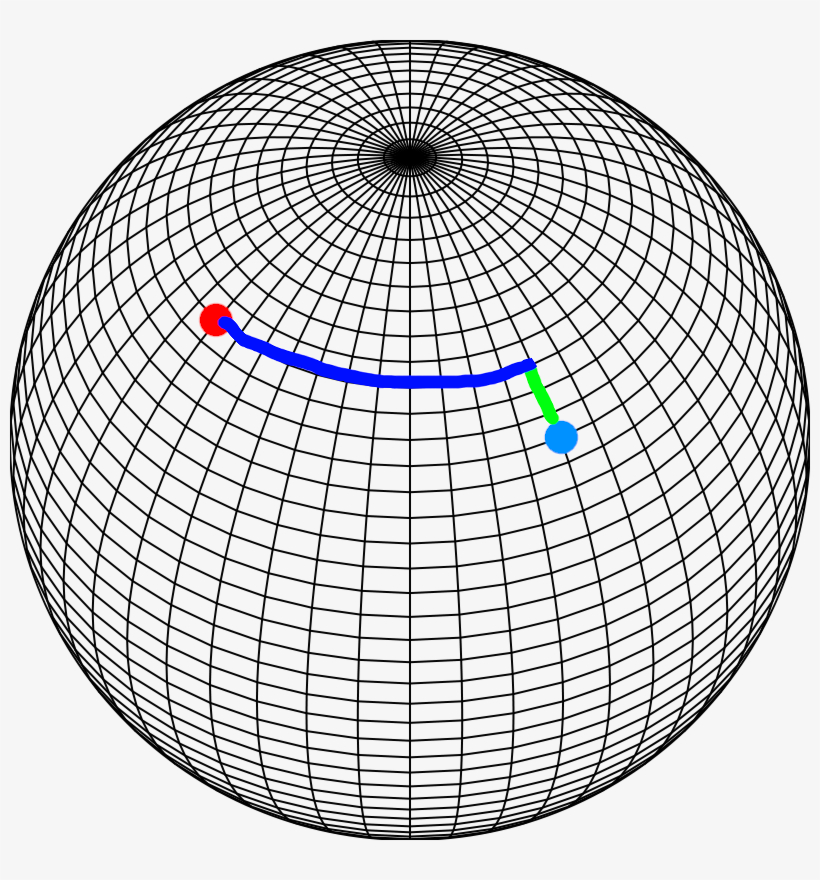
\includegraphics[width=0.7\linewidth]{img1.png}
        \caption*{Distance over shortest lateral circle plus longitudinal distance between points.}
    \end{subfigure}
    \begin{subfigure}[t]{0.49\linewidth}
        \centering
        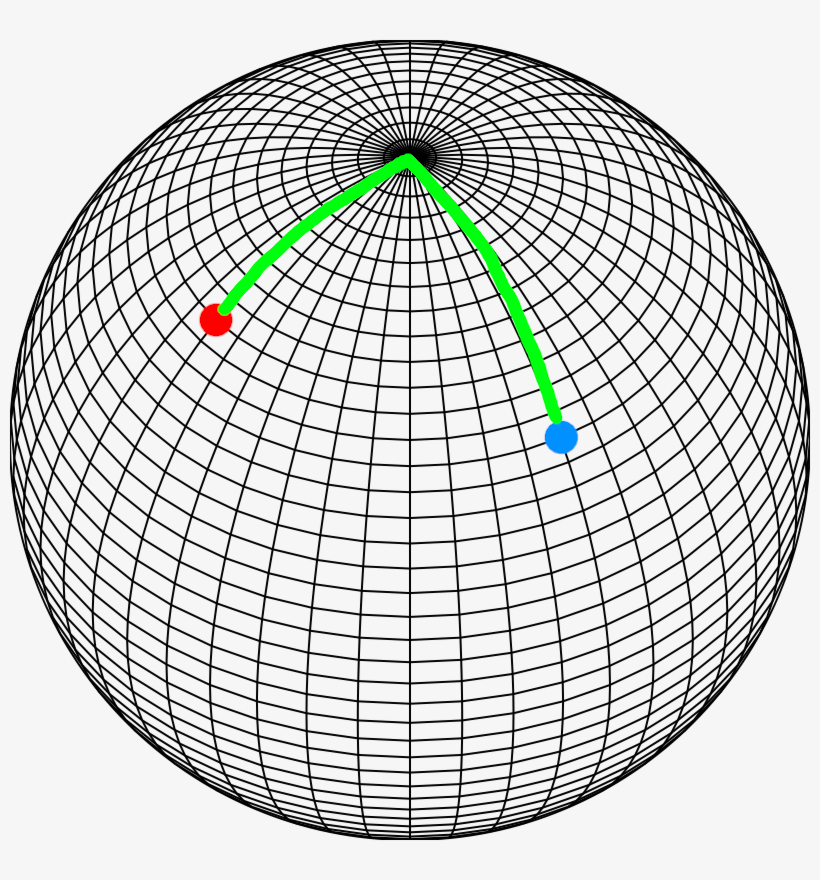
\includegraphics[width=0.7\linewidth]{img2.png}
        \caption*{Distance over north pole.}
    \end{subfigure}
\end{figure}

\section{Transform spherical to euclidean coordinates}

Transform a spherical point $p_s$ given as $p_s=(r,\theta, \varphi)$ to its euclidean representation $p_e=(x, y, z)$

\begin{align}
    x &= r \cdot \sin(\varphi) \cdot \cos(\theta)\\
    y &= r \cdot \sin(\varphi) \cdot \sin(\theta)\\
    z &= r \cdot \cos(\varphi) \\
    p_e &= (x, y, z)
\end{align}

\section{Transform euclidean to spherical coordinates}

Transform a euclidean point $p_e$ given as $p_e=(x, y, z)$ to its spherical representation $p_s=(r,\theta, \varphi)$

\begin{align}
    r &= \sqrt{x^2 + y^2 + z^2}\\
    \theta &= \tan^{-1}(\frac{y}{x})\\
    \varphi &= \cos^{-1}(\frac{z}{r}) \\
    p_s &= (r, \theta, \varphi)
\end{align}

\end{document}
